% Native editable composition from verified, unchanged IDE images.
\begin{figure}[htbp]
\centering
\sbox0{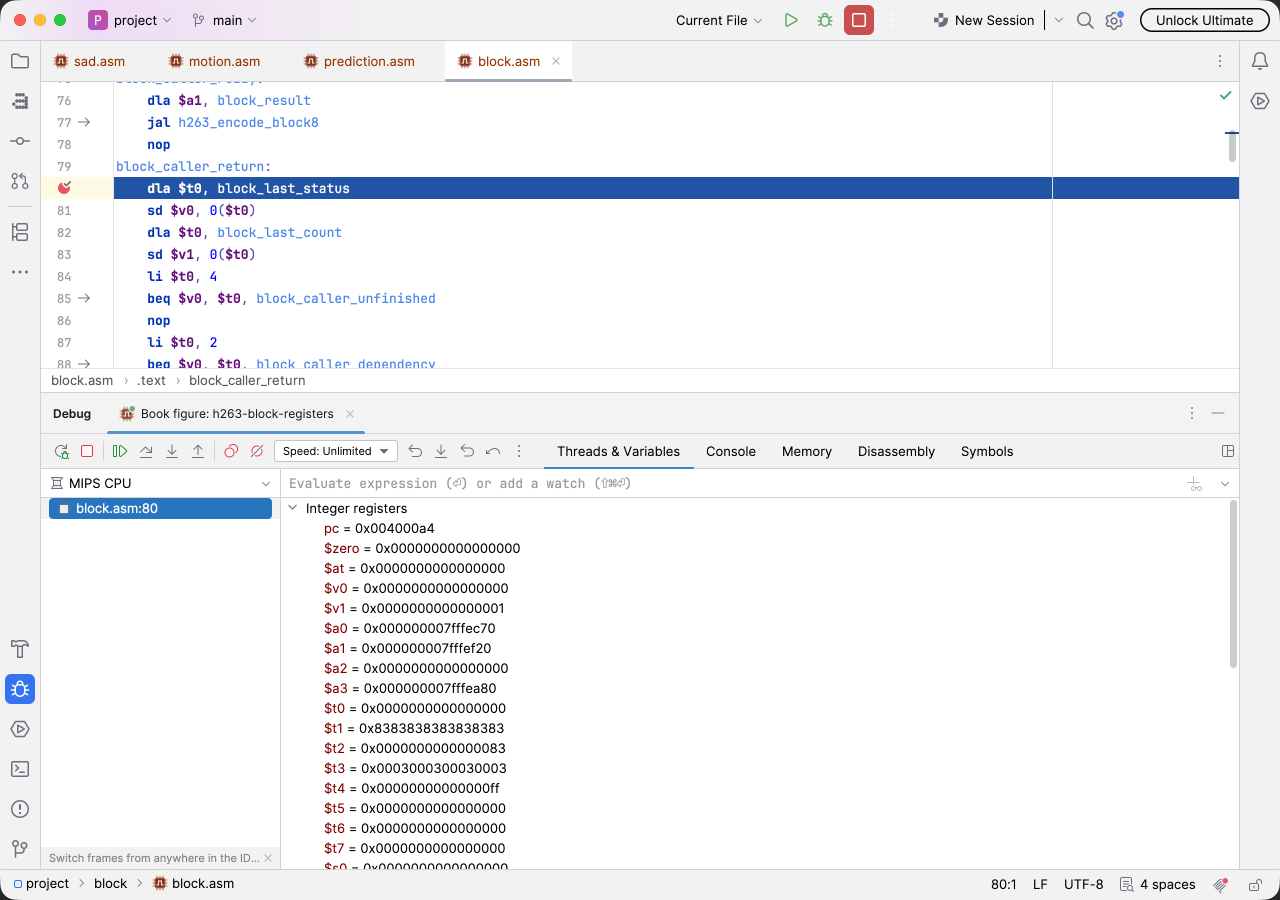
\includegraphics[artifact]{packages/035-h263/captures/h263-block-reconstruction/registers.png}}
\sbox2{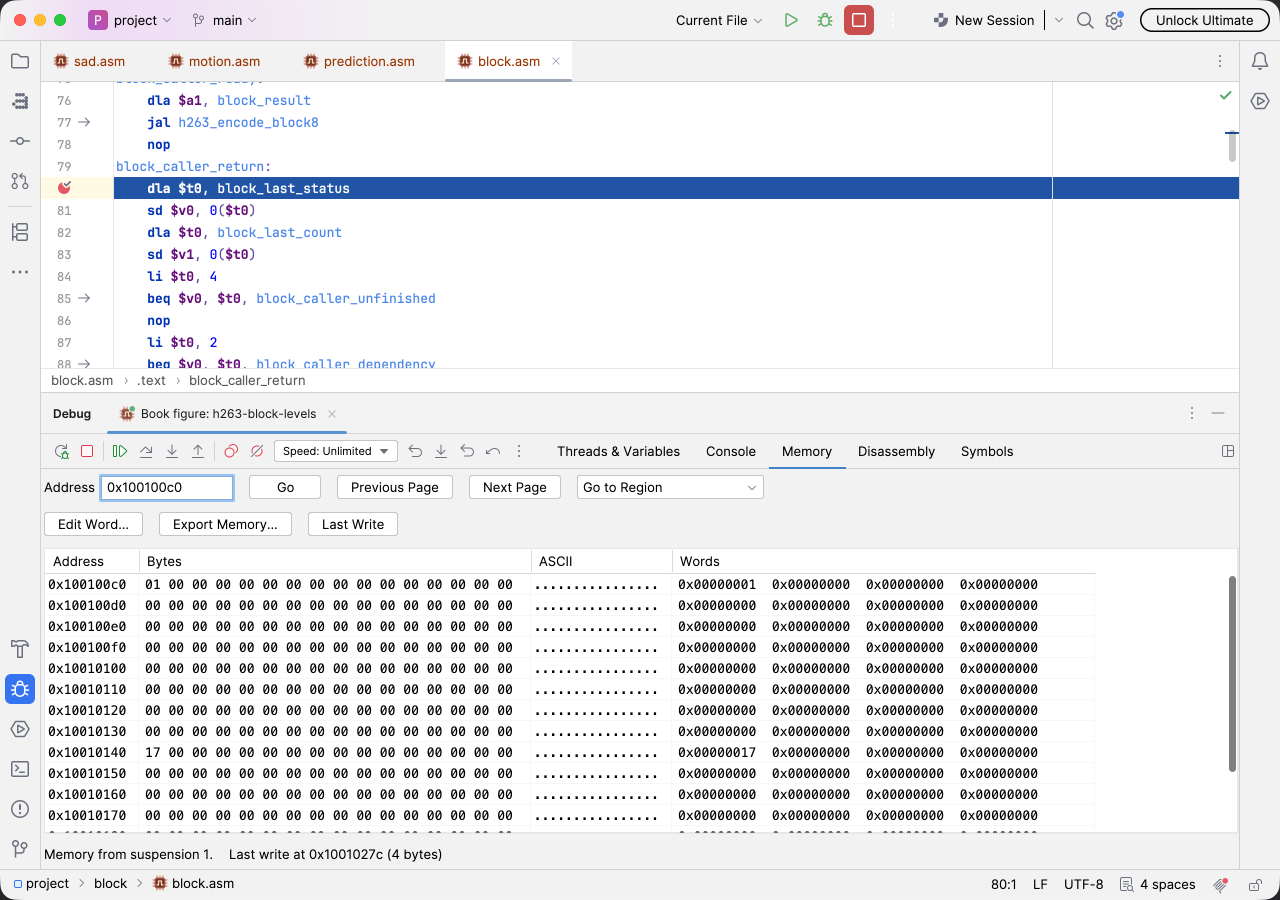
\includegraphics[artifact]{packages/035-h263/captures/h263-block-reconstruction/levels.png}}
\sbox4{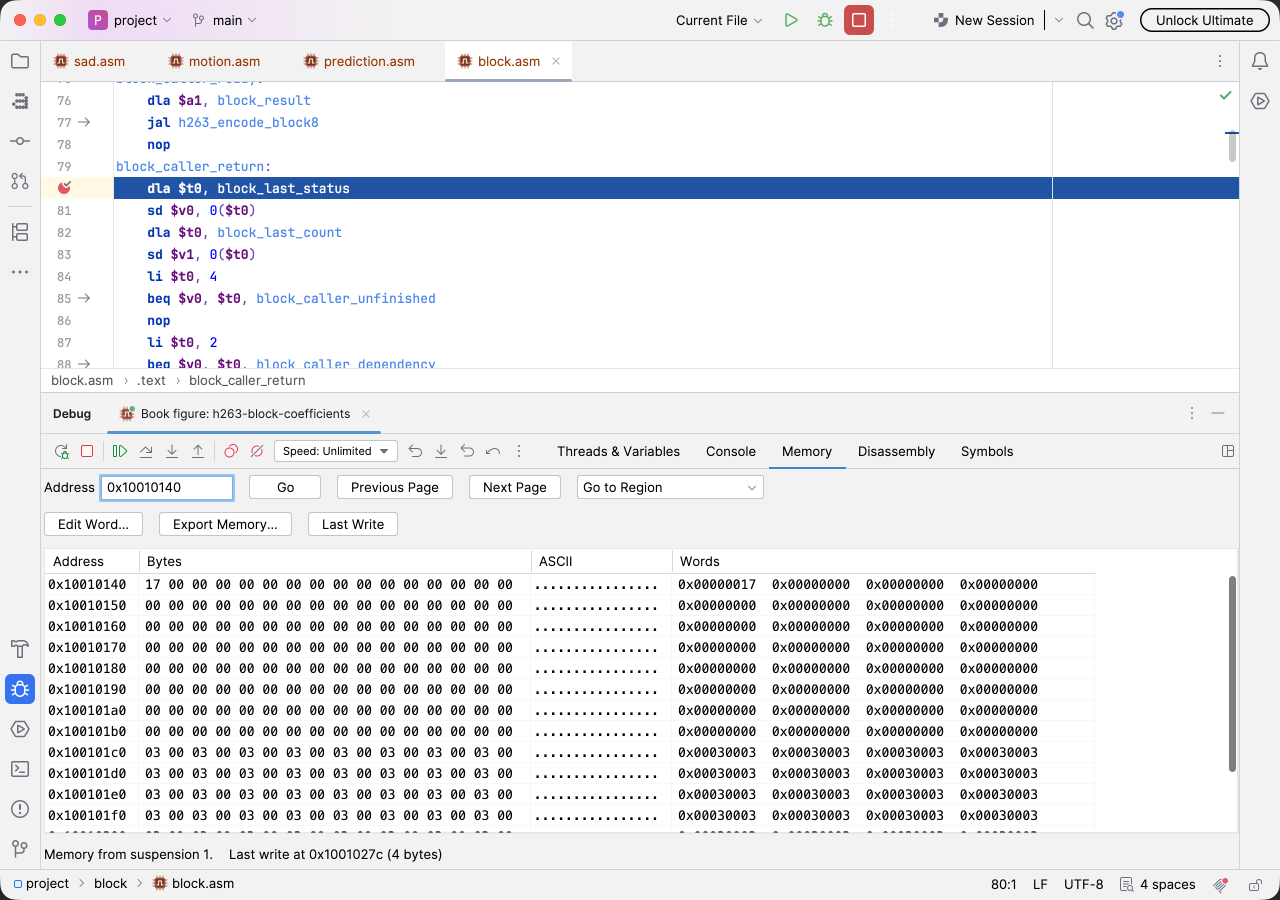
\includegraphics[artifact]{packages/035-h263/captures/h263-block-reconstruction/coefficients.png}}
\sbox6{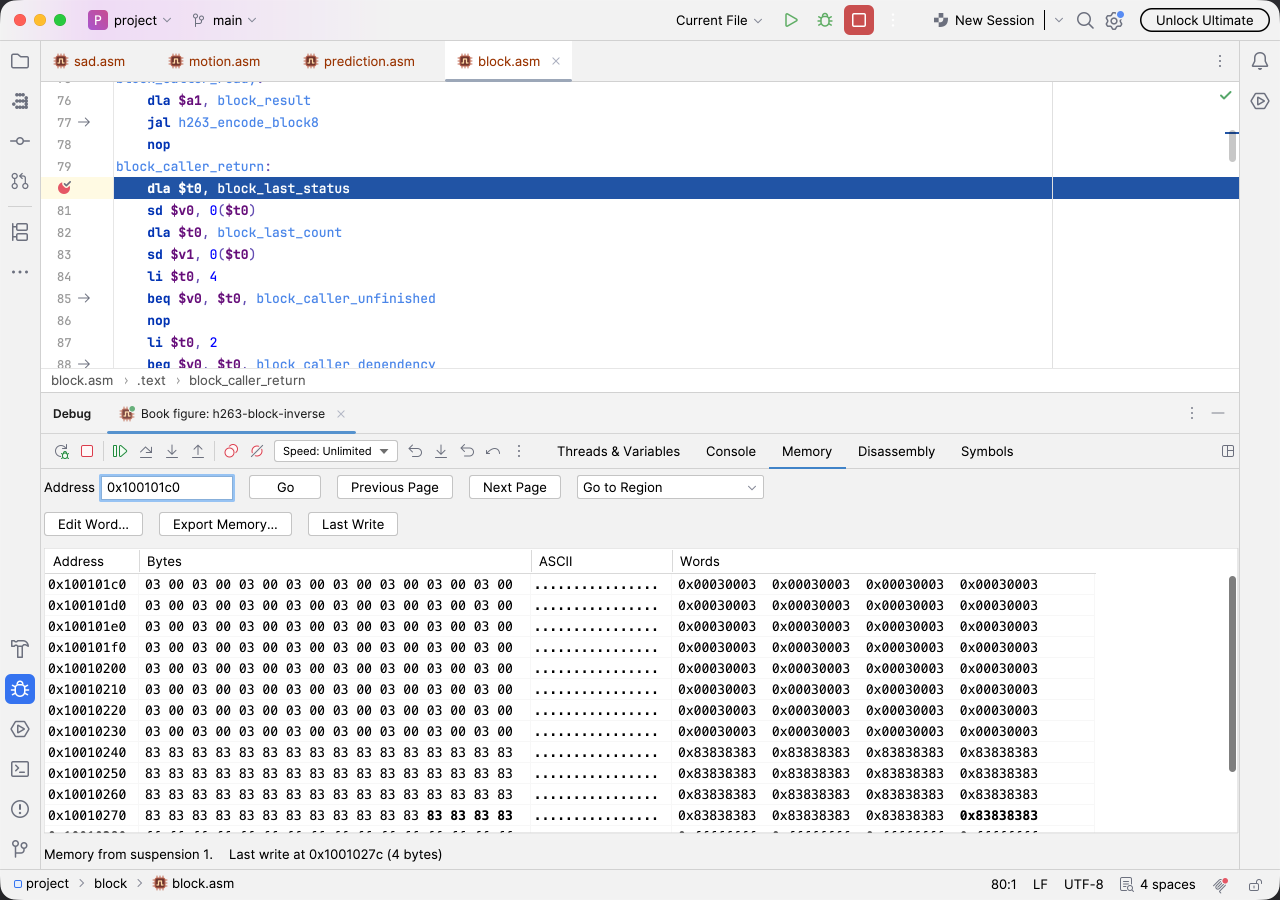
\includegraphics[artifact]{packages/035-h263/captures/h263-block-reconstruction/inverse.png}}
\sbox8{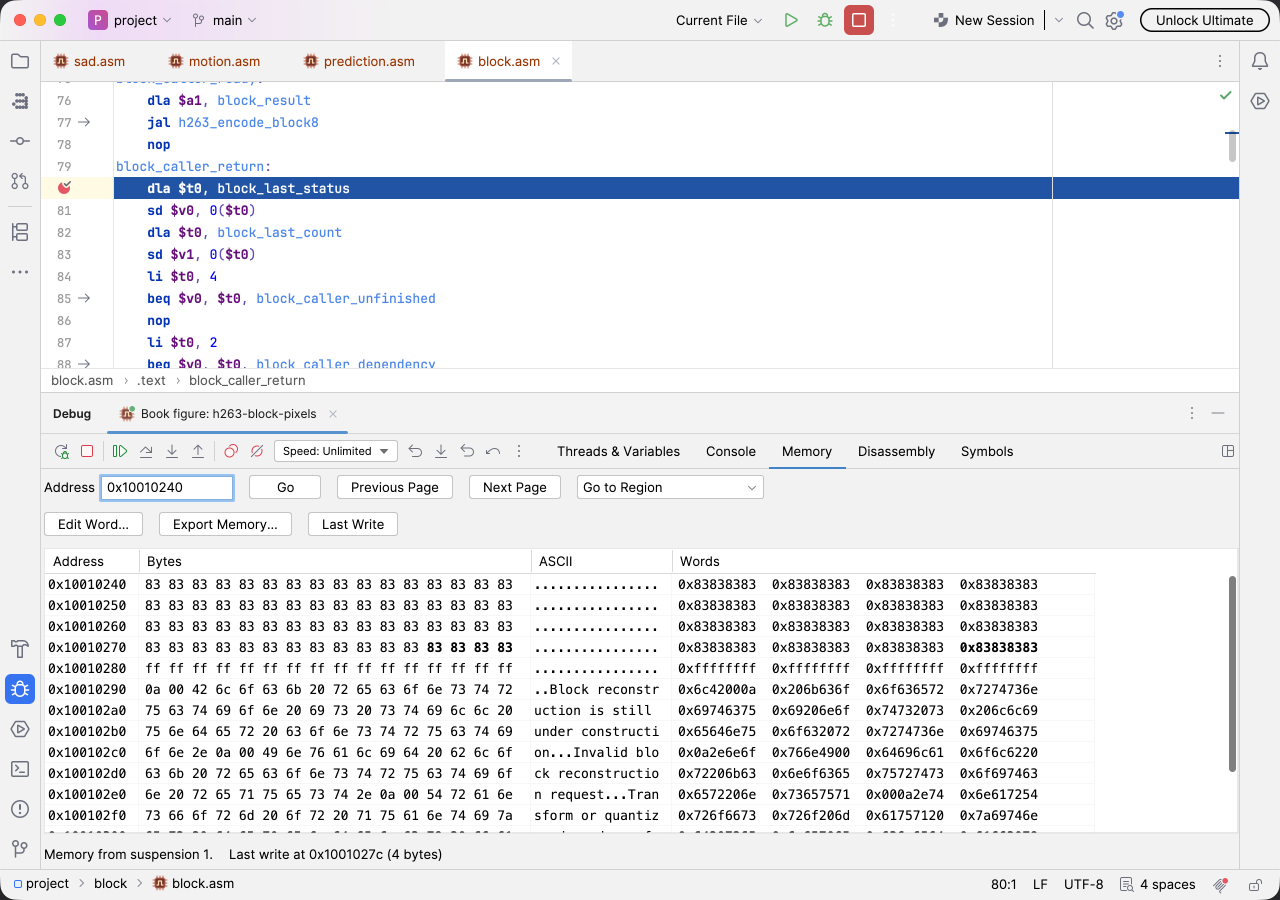
\includegraphics[artifact]{packages/035-h263/captures/h263-block-reconstruction/pixels.png}}
\edef\MARSblocksourceLeft{\the\dimexpr0.036718750\wd0\relax}
\edef\MARSblocksourceBottom{\the\dimexpr0.774444444\ht0\relax}
\edef\MARSblocksourceRight{\the\dimexpr0.611718750\wd0\relax}
\edef\MARSblocksourceTop{\the\dimexpr0.170000000\ht0\relax}
\edef\MARSblocklevelsLeft{\the\dimexpr0.108593750\wd2\relax}
\edef\MARSblocklevelsBottom{\the\dimexpr0.335555556\ht2\relax}
\edef\MARSblocklevelsRight{\the\dimexpr0.585156250\wd2\relax}
\edef\MARSblocklevelsTop{\the\dimexpr0.634444444\ht2\relax}
\edef\MARSblockcoefficientsLeft{\the\dimexpr0.108593750\wd4\relax}
\edef\MARSblockcoefficientsBottom{\the\dimexpr0.335555556\ht4\relax}
\edef\MARSblockcoefficientsRight{\the\dimexpr0.585156250\wd4\relax}
\edef\MARSblockcoefficientsTop{\the\dimexpr0.634444444\ht4\relax}
\edef\MARSblockinverseLeft{\the\dimexpr0.108593750\wd6\relax}
\edef\MARSblockinverseBottom{\the\dimexpr0.335555556\ht6\relax}
\edef\MARSblockinverseRight{\the\dimexpr0.585156250\wd6\relax}
\edef\MARSblockinverseTop{\the\dimexpr0.634444444\ht6\relax}
\edef\MARSblockpixelsLeft{\the\dimexpr0.108593750\wd8\relax}
\edef\MARSblockpixelsBottom{\the\dimexpr0.335555556\ht8\relax}
\edef\MARSblockpixelsRight{\the\dimexpr0.585156250\wd8\relax}
\edef\MARSblockpixelsTop{\the\dimexpr0.634444444\ht8\relax}
\edef\MARSblockreturnsLeft{\the\dimexpr0.246093750\wd0\relax}
\edef\MARSblockreturnsBottom{\the\dimexpr0.310000000\ht0\relax}
\edef\MARSblockreturnsRight{\the\dimexpr0.596875000\wd0\relax}
\edef\MARSblockreturnsTop{\the\dimexpr0.638888889\ht0\relax}
\begin{tikzpicture}[alt={Six annotated details at block_caller_return. Status v0 is zero and ordinary nonzero level count v1 is one. The level array begins 01 00. Reconstructed coefficients at offset 128 begin 17 00, decimal 23. Inverse residuals at offset 256 contain 03 00 halfwords. Reconstructed pixel bytes at offset 384 contain 83, decimal 131. The highlighted dla precedes the caller stores.}]
\node[anchor=north west,inner sep=0,font=\small\bfseries] (source-title) at (6mm,0) {Completed block before caller bookkeeping};
\node[anchor=north west,inner sep=0] (source) at ([yshift=-1mm]source-title.south west) {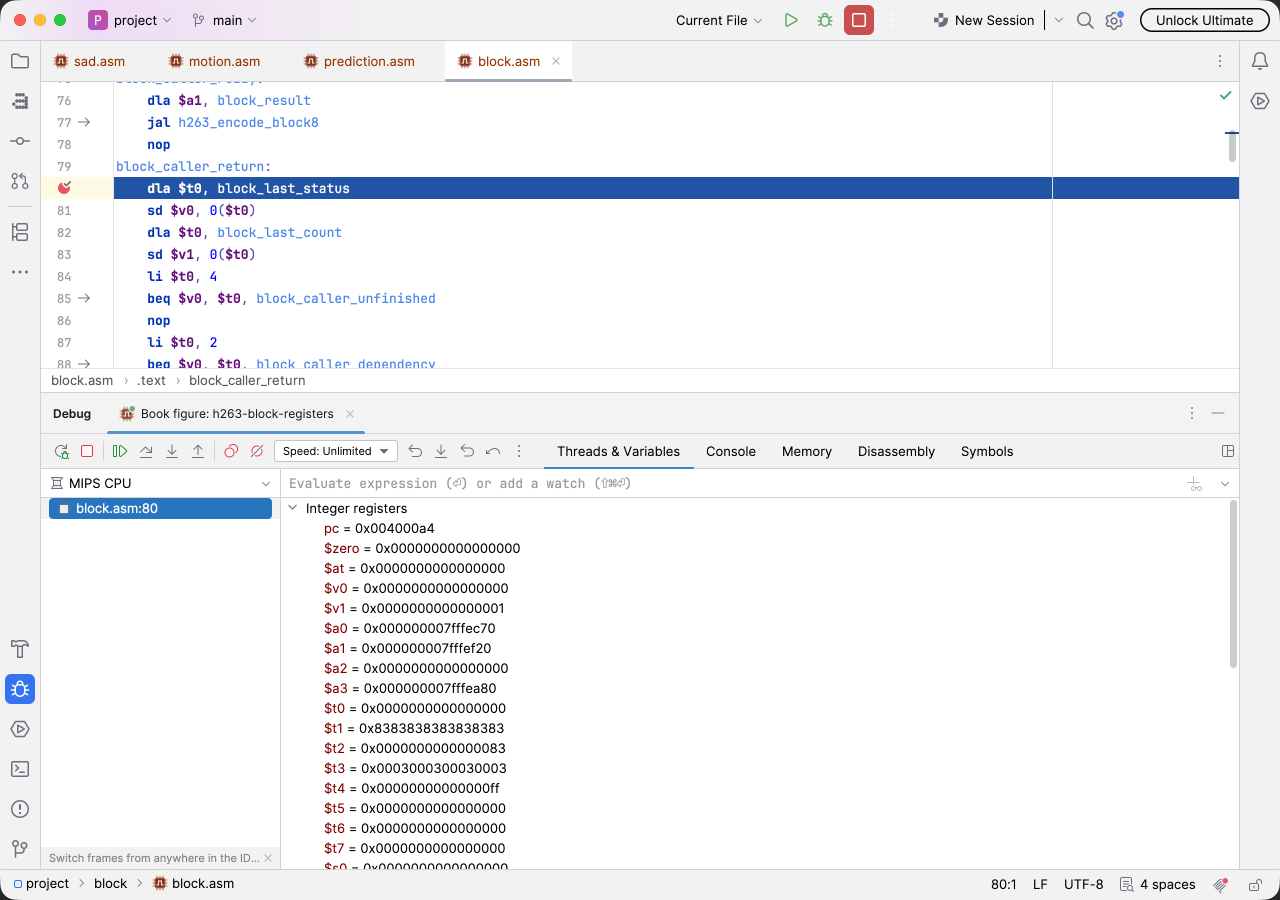
\includegraphics[width=0.7\linewidth,artifact,trim={\MARSblocksourceLeft{} \MARSblocksourceBottom{} \MARSblocksourceRight{} \MARSblocksourceTop{}},clip]{packages/035-h263/captures/h263-block-reconstruction/registers.png}};
\begin{scope}[shift={(source.south west)},x={($(source.south east)-(source.south west)$)},y={($(source.north west)-(source.south west)$)}]
\draw[black,line width=0.7pt] (0.153333333,0.080000000) rectangle (0.673333333,0.520000000);
\node[draw=black,fill=white,circle,inner sep=1.5pt,font=\footnotesize] at ($(0.153333333,0.520000000)+(-3mm,0)$) {1};
\end{scope}
\node[anchor=north west,inner sep=0,font=\small\bfseries] (levels-title) at ([yshift=-2mm]source.south west) {Selected levels at result offset zero};
\node[anchor=north west,inner sep=0] (levels) at ([yshift=-1mm]levels-title.south west) {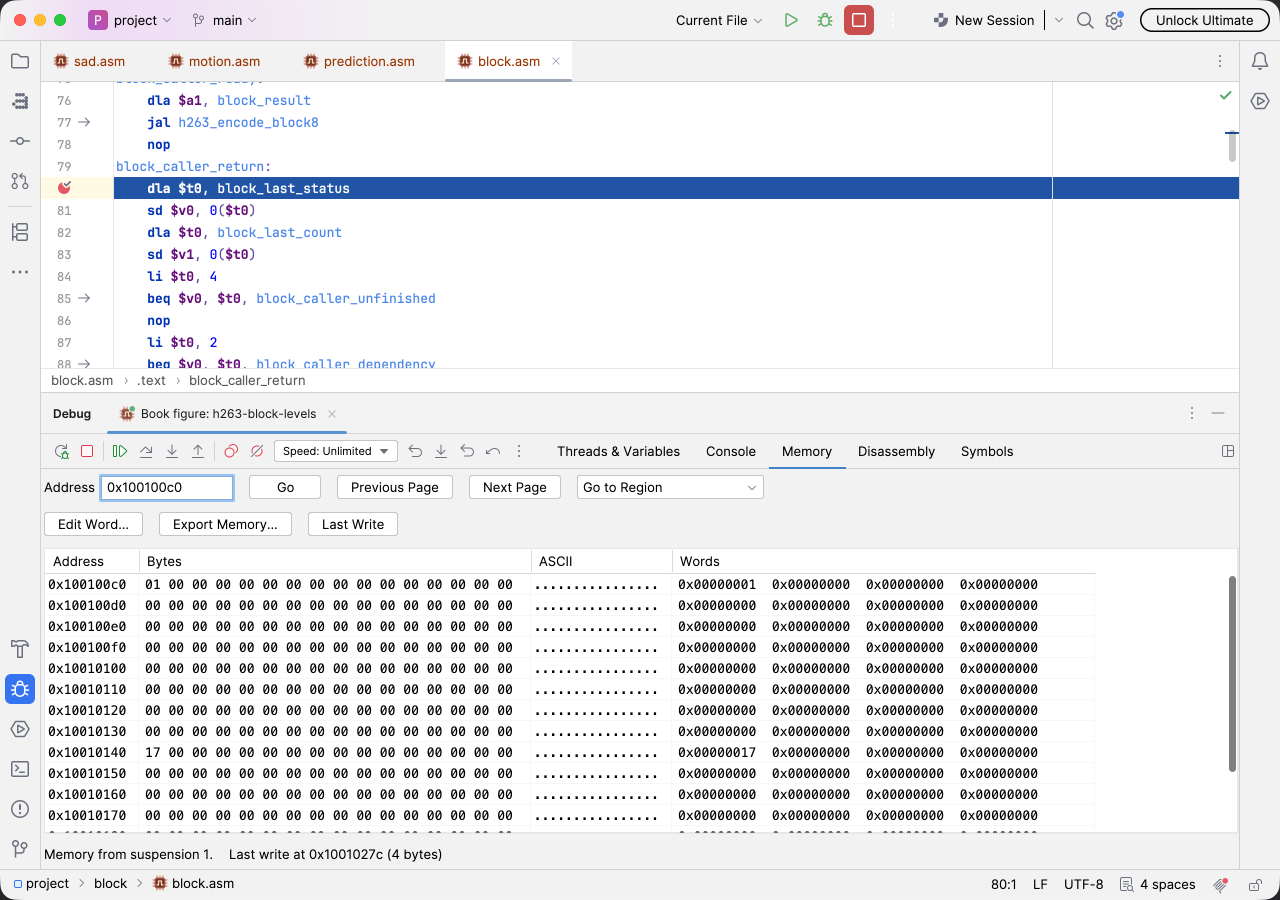
\includegraphics[width=0.84\linewidth,artifact,trim={\MARSblocklevelsLeft{} \MARSblocklevelsBottom{} \MARSblocklevelsRight{} \MARSblocklevelsTop{}},clip]{packages/035-h263/captures/h263-block-reconstruction/levels.png}};
\begin{scope}[shift={(levels.south west)},x={($(levels.south east)-(levels.south west)$)},y={($(levels.north west)-(levels.south west)$)}]
\draw[black,line width=0.7pt] (0.000000000,0.111111111) rectangle (1.000000000,0.888888889);
\node[draw=black,fill=white,circle,inner sep=1.5pt,font=\footnotesize] at ($(0.000000000,0.888888889)+(-3mm,0)$) {2};
\end{scope}
\node[anchor=north west,inner sep=0,font=\small\bfseries] (coefficients-title) at ([yshift=-2mm]levels.south west) {Reconstructed coefficients at offset 128};
\node[anchor=north west,inner sep=0] (coefficients) at ([yshift=-1mm]coefficients-title.south west) {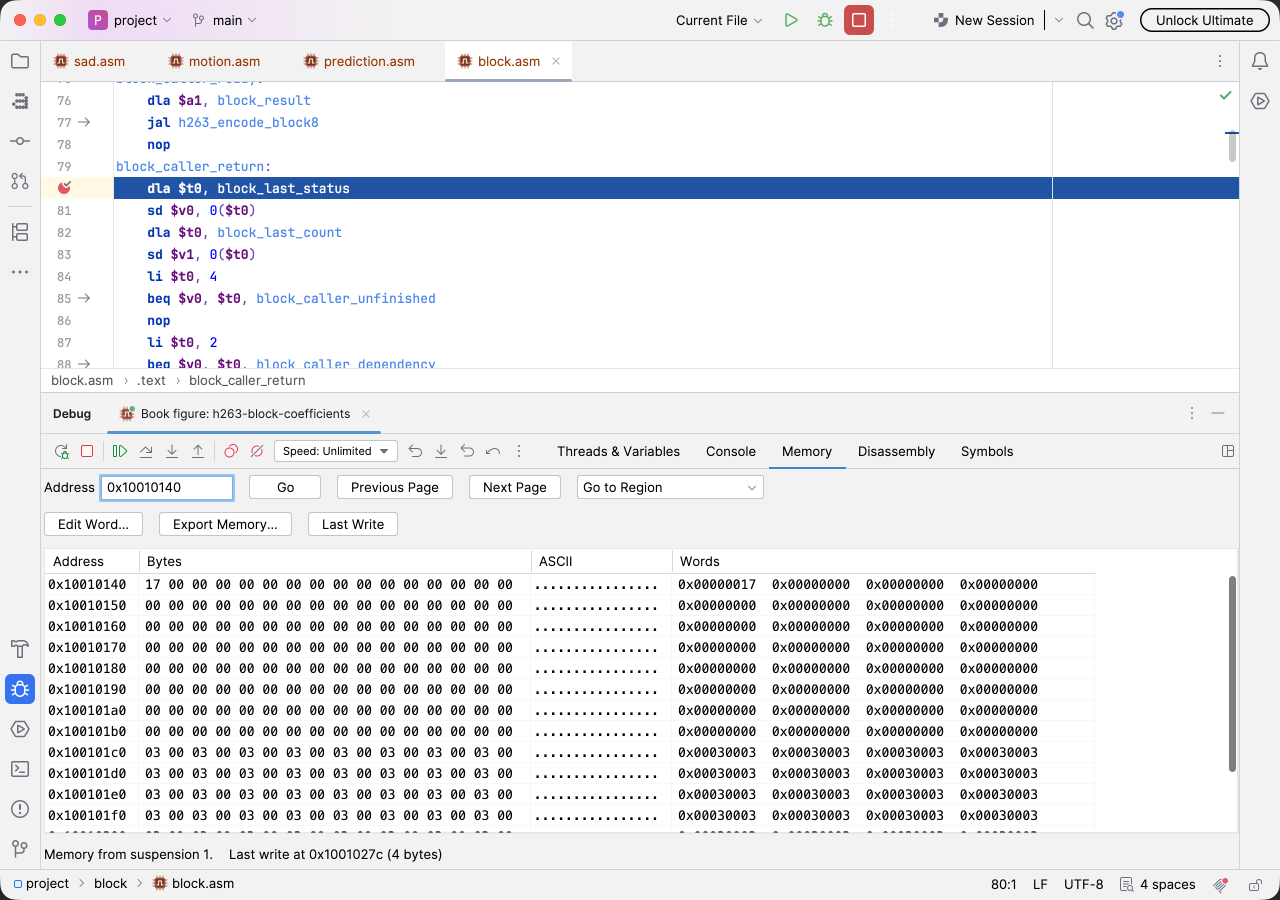
\includegraphics[width=0.84\linewidth,artifact,trim={\MARSblockcoefficientsLeft{} \MARSblockcoefficientsBottom{} \MARSblockcoefficientsRight{} \MARSblockcoefficientsTop{}},clip]{packages/035-h263/captures/h263-block-reconstruction/coefficients.png}};
\begin{scope}[shift={(coefficients.south west)},x={($(coefficients.south east)-(coefficients.south west)$)},y={($(coefficients.north west)-(coefficients.south west)$)}]
\draw[black,line width=0.7pt] (0.000000000,0.111111111) rectangle (1.000000000,0.888888889);
\node[draw=black,fill=white,circle,inner sep=1.5pt,font=\footnotesize] at ($(0.000000000,0.888888889)+(-3mm,0)$) {3};
\end{scope}
\node[anchor=north west,inner sep=0,font=\small\bfseries] (inverse-title) at ([yshift=-2mm]coefficients.south west) {Inverse residuals at offset 256};
\node[anchor=north west,inner sep=0] (inverse) at ([yshift=-1mm]inverse-title.south west) {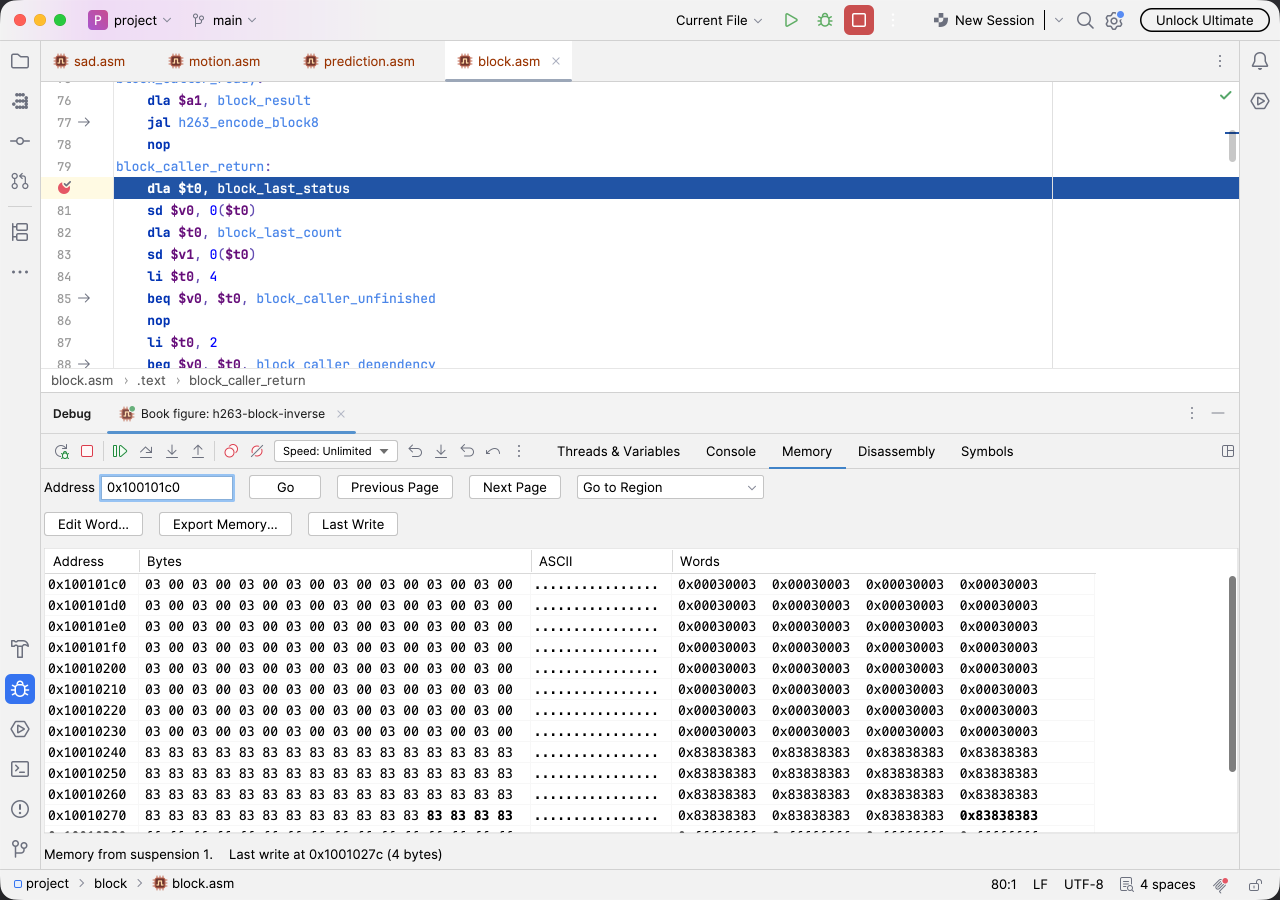
\includegraphics[width=0.84\linewidth,artifact,trim={\MARSblockinverseLeft{} \MARSblockinverseBottom{} \MARSblockinverseRight{} \MARSblockinverseTop{}},clip]{packages/035-h263/captures/h263-block-reconstruction/inverse.png}};
\begin{scope}[shift={(inverse.south west)},x={($(inverse.south east)-(inverse.south west)$)},y={($(inverse.north west)-(inverse.south west)$)}]
\draw[black,line width=0.7pt] (0.000000000,0.111111111) rectangle (1.000000000,0.888888889);
\node[draw=black,fill=white,circle,inner sep=1.5pt,font=\footnotesize] at ($(0.000000000,0.888888889)+(-3mm,0)$) {4};
\end{scope}
\node[anchor=north west,inner sep=0,font=\small\bfseries] (pixels-title) at ([yshift=-2mm]inverse.south west) {Reconstructed pixels at offset 384};
\node[anchor=north west,inner sep=0] (pixels) at ([yshift=-1mm]pixels-title.south west) {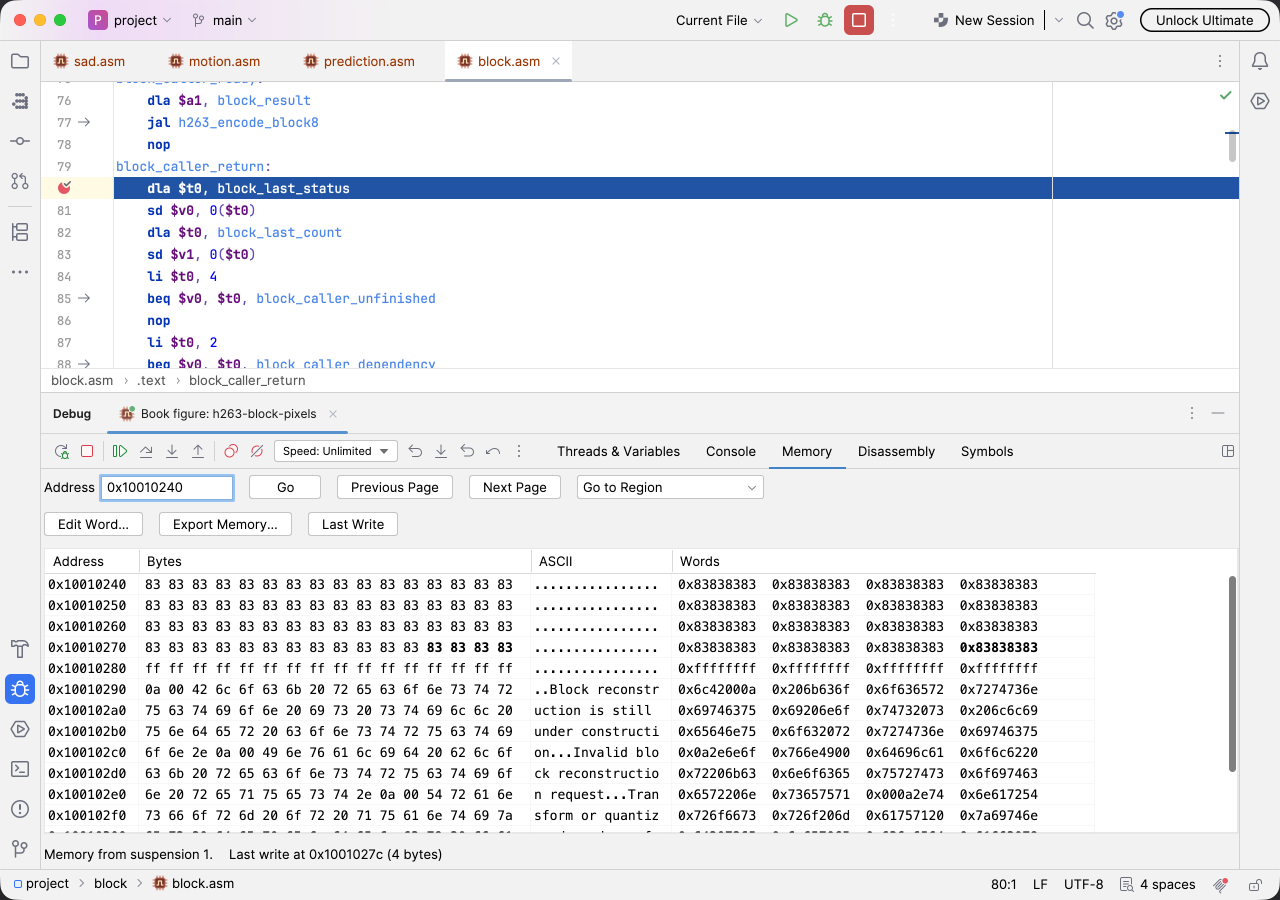
\includegraphics[width=0.84\linewidth,artifact,trim={\MARSblockpixelsLeft{} \MARSblockpixelsBottom{} \MARSblockpixelsRight{} \MARSblockpixelsTop{}},clip]{packages/035-h263/captures/h263-block-reconstruction/pixels.png}};
\begin{scope}[shift={(pixels.south west)},x={($(pixels.south east)-(pixels.south west)$)},y={($(pixels.north west)-(pixels.south west)$)}]
\draw[black,line width=0.7pt] (0.000000000,0.111111111) rectangle (1.000000000,0.888888889);
\node[draw=black,fill=white,circle,inner sep=1.5pt,font=\footnotesize] at ($(0.000000000,0.888888889)+(-3mm,0)$) {5};
\end{scope}
\node[anchor=north west,inner sep=0,font=\small\bfseries] (returns-title) at ([yshift=-2mm]pixels.south west) {Successful block and ordinary nonzero count};
\node[anchor=north west,inner sep=0] (returns) at ([yshift=-1mm]returns-title.south west) {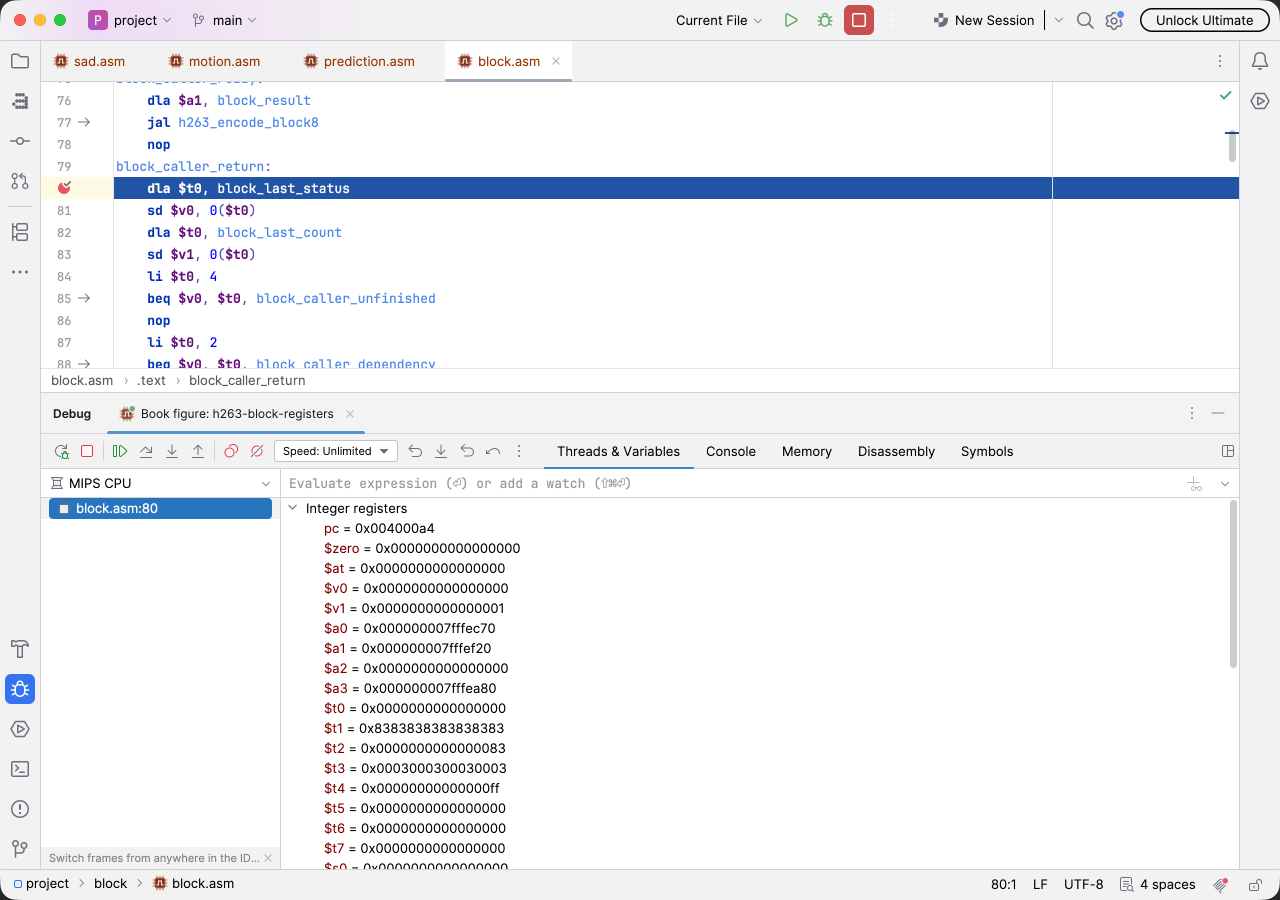
\includegraphics[width=0.5\linewidth,artifact,trim={\MARSblockreturnsLeft{} \MARSblockreturnsBottom{} \MARSblockreturnsRight{} \MARSblockreturnsTop{}},clip]{packages/035-h263/captures/h263-block-reconstruction/registers.png}};
\begin{scope}[shift={(returns.south west)},x={($(returns.south east)-(returns.south west)$)},y={($(returns.north west)-(returns.south west)$)}]
\draw[black,line width=0.7pt] (0.029850746,0.065217391) rectangle (0.970149254,0.934782609);
\node[draw=black,fill=white,circle,inner sep=1.5pt,font=\footnotesize] at ($(0.029850746,0.934782609)+(-3mm,0)$) {6};
\end{scope}
\end{tikzpicture}
\par\smallskip
\begin{minipage}{\linewidth}
\small
\begin{enumerate}
\item The result is the default INTER example: current samples 130, prediction samples 128 and $Q=8$. The routine has returned before the caller records its status.
\item The first signed halfword is level one, stored as \texttt{01 00}. The remaining levels in this first row are zero.
\item The selected level reconstructs to coefficient 23, stored as \texttt{17 00}. This array is derived from the selected levels rather than copied from the forward transform.
\item The inverse transform produces residual three, represented by \texttt{03 00} halfwords. This is the residual used to construct the future reference picture.
\item Adding prediction 128 gives pixel 131, stored as byte \texttt{83}. It differs from the raw input 130 because the encoder reconstructs the quantized representation that a decoder receives.
\item \texttt{\$v0}=0 and \texttt{\$v1}=1. The count describes ordinary nonzero quantized levels; it is neither a pixel count nor the reconstructed DC value.
\end{enumerate}
\end{minipage}
\caption{The default INTER block reconstructed from its selected levels. Five Debug launches inspect one source and return checkpoint.}
\label{fig:h263-block-reconstruction}
\end{figure}
